\documentclass{article}
\usepackage{amsmath}
\usepackage{listings}
\usepackage[utf8]{inputenc}
\usepackage{graphicx}

\lstset{
	basicstyle=\footnotesize,
	numbers=left,
	tabsize=3,
	title=\lstname,
	breaklines=true
}

\addtolength{\oddsidemargin}{-.875in}
\addtolength{\evensidemargin}{-.875in}
\addtolength{\textwidth}{1.75in}

\addtolength{\topmargin}{-.875in}
\addtolength{\textheight}{1.75in}
	
	
\begin{document}
\section*{Übung 4 - Neuronale Netze}
\subsection*{Tobias Hahn - 3073375}
\section{Perzeptionsalgorithmus}
\subsection{Implementierung}
\paragraph{}
Ich habe den Algorithmus in zwei Klassen implementiert, perception.py und training.py. Die erste Klasse liefert dabei alle notwendigen Methoden, um aus einem Datenset mit mitgelieferter Klassifizierung einen Trennungsvektor zu ermitteln. Dabei wurde der verbesserte Additions- bzw. Subtraktionsalgorithmus verwendert, um eine verschnellerte Konvergenz zu erreichen.

\paragraph{}
Die zweite Klasse implementiert die Erstellung des zufälligen Datensets plus Ergebnissen, gibt einige Kenndaten über die Lösung aus und schlussendlich auch noch den Graphen.

\paragraph{}
Der Graph ist ein sogenannter Parallel Coordinates Graph, dabei wird für jede Dimension eine y-Achse erstellt, die einzelnen Datenpunkte sind Linien die durch die Werte auf den jeweiligen y-Achsen (Dimensionen) definiert werden. Jede Klasse ist hierbei durch die Farbe der Linien definiert.
Um die Übereinstimmung des gelernten Vektors mit dem ursprünglichen zu zeigen, wurde außerdem noch eine Dimension eingeführt, die die ursprüngliche Klassifizierung anzeigt. Hier müsste ien guter Algorithmus dafür sorgen, dass alle Linien einer Farbe sich auf einen Punkt vereinen - der in der Vorlesung vorgestellte Algorithmus leistet dies auch, wie man an den Ergebnissen sieht.

\paragraph{}
Im folgenden zuerst der Quellcode für die beiden Klassen, und danach das Bild mit dem Graphen welcher die Ergebnisse dokumentiert.
\paragraph{}
\lstinputlisting[language=Python]{../perceptron.py}
\lstinputlisting[language=Python]{../training.py}
\begin{lstlisting}[title=Beispielausgabe]
The original weight vector: [ 9.84658028  0.96802249 -8.5146963   1.333602   -3.55325839 -4.77932809 -0.08857396 -0.15751875 -6.47169592  7.71299722]
The learned vector: [  4.22755294e-04   1.77767972e-05  -3.40020042e-04   6.74635191e-05  -1.62867848e-04  -1.92920237e-04  -2.40298543e-05  -1.96774406e-05  -2.33433280e-04   3.34287987e-04]
The number of wrong classifications: 0
The number of adjustments made to the vector: 212
The total number of test iterations: 5446
\end{lstlisting}

\begin{figure}[h]
\caption{Graph des Datensets}
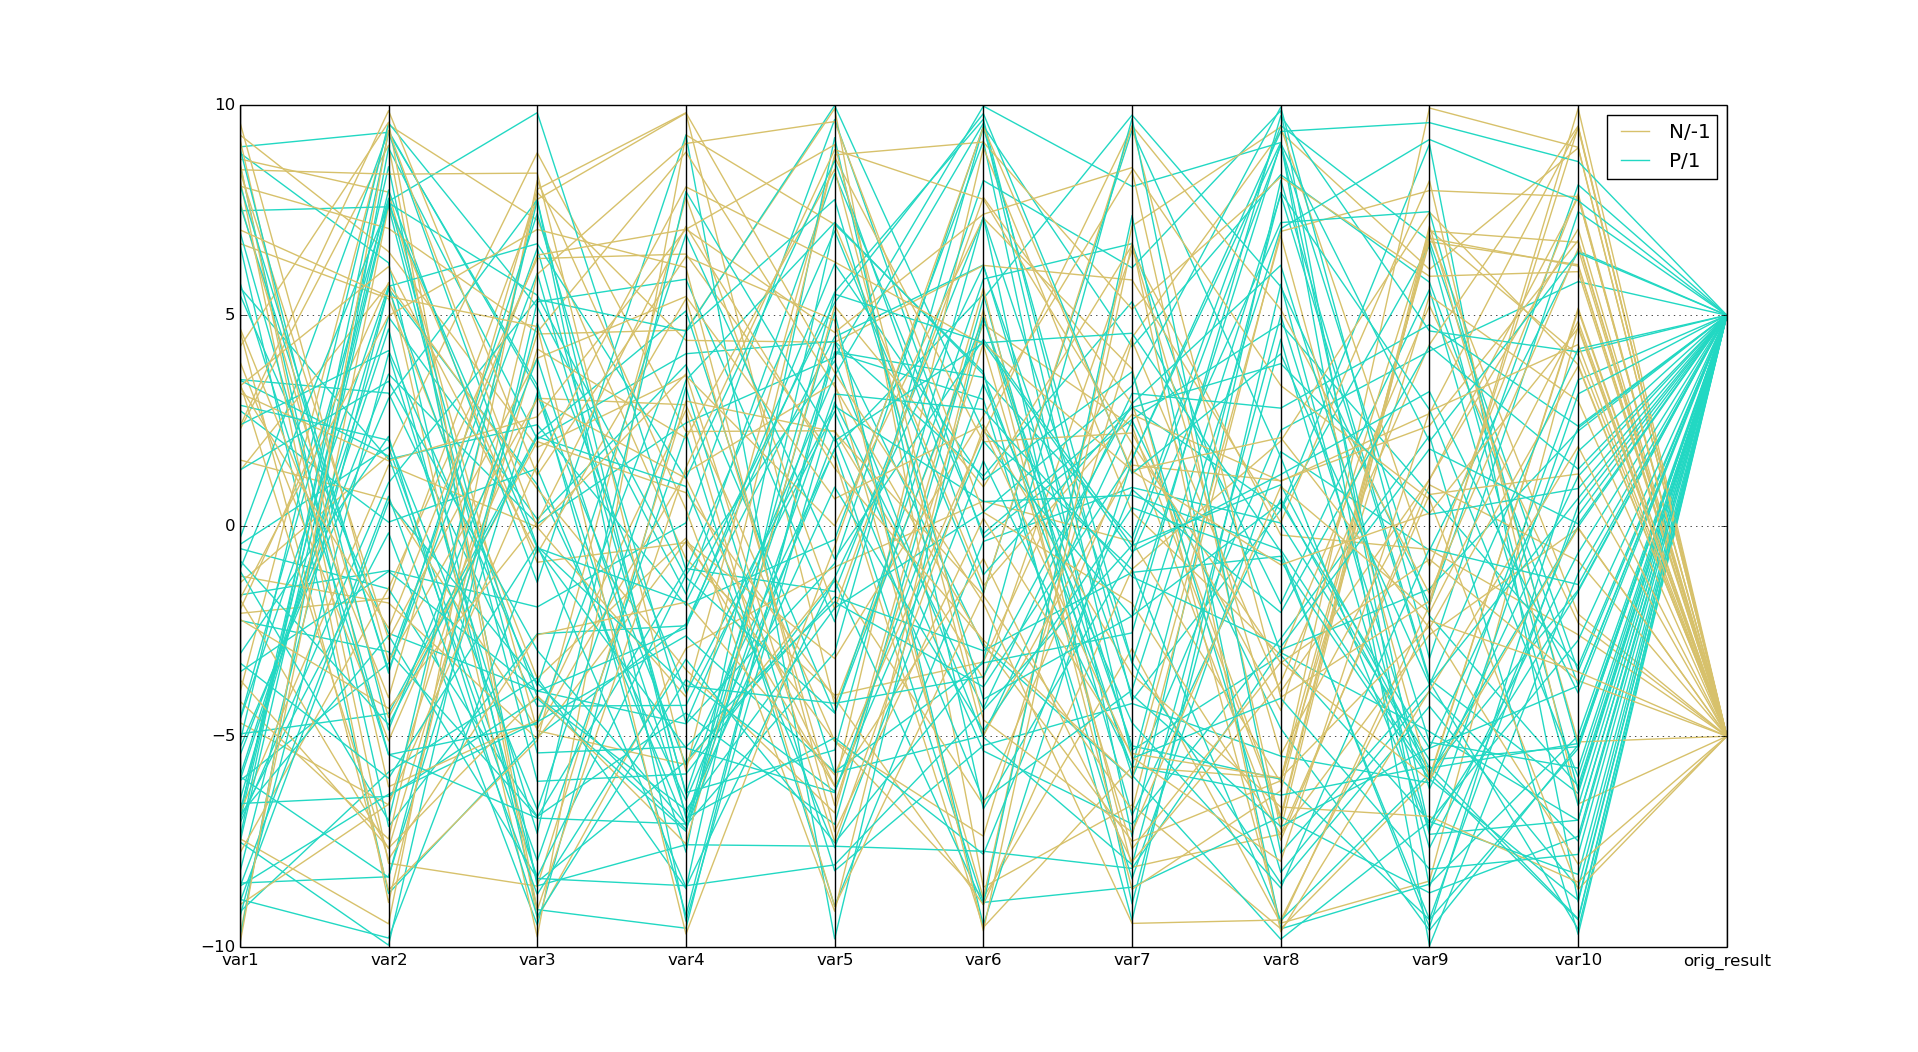
\includegraphics[width=\textwidth]{../graph}
\end{figure}

\subsection{Verständnisfrage}
\paragraph{}
Der Perzeptionsalgorithmus braucht für Konvergenz recht lange, wenn zwei Datenpunkte antiparallel sind. Zwei Vektoren sind dann antiparallel, wenn einer der beiden Vektoren das Produkt des anderen mit einer negativen Zahl ist.

\paragraph{}
Um dies zu begründen stellen wir die beiden Vektoren zuerst als Summe dreier anderer Vektoren dar:

\begin{alignat*}{1}
	x &=  g + x_{diff} \\
	y &=  -g + y_{diff}
\end{alignat*}

\paragraph{}
Wobei wir festhalten können dass die beiden Anteile die hinter g stehen jeweils ziemlich klein sind, da die Vektoren ja fast antiparallell sind. Nun würde der Algorithmus bei jeder Iteration abwechselnd g zum Gewichtsvektor hinzufügen und wieder abziehen, was sich im Mittel ausgleicht. Lediglich der kleine Differenzvektor würde den Gewichtsvektor in die "richtige" Richtung bringen, da nur dieser den Unterschied zwischen x und y ausmacht. Je kleiner dieser Differenzvektor, je "antiparalleler" die Vektoren also sind, desto weniger bewegt sich der Gewichtsvektor also in die richtige Richtung mit jeder Iteration.

\subsubsection{Beispieldaten}
\begin{tabular}{|l|l|l|l|}
	\hline
	Dimensionen & Vektor x & Vektor y \\\hline
	x & 1.01 & -1.02 \\\hline
	y & 1.01 & -1.02 \\\hline
\end{tabular}
\end{document}
